\documentclass{exam}
\usepackage{algpseudocode}
\usepackage{algorithm}
\usepackage{amsmath}

\usepackage{indentfirst}
\usepackage{graphicx}
\usepackage{listings}
\usepackage{color}
\usepackage{fancyvrb}

\definecolor{mygreen}{rgb}{0,0.6,0}
\definecolor{mygray}{rgb}{0.5,0.5,0.5}
\definecolor{mymauve}{rgb}{0.58,0,0.82}

\lstset{ %
	backgroundcolor=\color{white},		% choose the background color; you must add \usepackage{color} or \usepackage{xcolor}
	basicstyle=\small\ttfamily,		% the size of the fonts that are used for the code
	breakatwhitespace=false,			% sets if automatic breaks should only happen at whitespace
	breaklines=true,					% sets automatic line breaking
	captionpos=b,						% sets the caption-position to bottom
	columns=fullflexible,
	commentstyle=\color{mygreen},		% comment style
	deletekeywords={...},				% if you want to delete keywords from the given language
	escapeinside={\%*}{*)},			% if you want to add LaTeX within your code
	extendedchars=true,				% lets you use non-ASCII characters; for 8-bits encodings only, does not work with UTF-8
	frame=single,						% adds a frame around the code
	keepspaces=true,					% keeps spaces in text, useful for keeping indentation of code (possibly needs columns=flexible)
	keywordstyle=\color{blue},			% keyword style
	language=Octave,					% the language of the code
	morekeywords={*,...},				% if you want to add more keywords to the set
	%   numbers=left,						% where to put the line-numbers; possible values are (none, left, right)
	%   numbersep=6pt,						% how far the line-numbers are from the code
	%   numberstyle=\tiny\color{mygray},	% the style that is used for the line-numbers
	rulecolor=\color{black},			% if not set, the frame-color may be changed on line-breaks within not-black text (e.g. comments (green here))
	showspaces=false,					% show spaces everywhere adding particular underscores; it overrides 'showstringspaces'
	showstringspaces=false,			% underline spaces within strings only
	showtabs=false,					% show tabs within strings adding particular underscores
	stepnumber=1,						% the step between two line-numbers. If it's 1, each line will be numbered
	stringstyle=\color{mymauve},		% string literal style
	tabsize=2,							% sets default tabsize to 2 spaces
	title=\lstname						% show the filename of files included with \lstinputlisting; also try caption instead of title
}

% Creates a new command to include a perl script, the first parameter is the filename of the script (without .pl), the second parameter is the caption
\newcommand{\octavescript}[2]{
	\lstinputlisting[caption=#2]{#1}
}

\newcommand{\MNLab}{Laborator\ \#6}
\newcommand{\MNLabTitle}{Soluția ecuației neliniare $f(x)=0$. Analiza convergenței. Lucrul cu polinoame în MATLAB. Rezolvarea sistemelor de ecuații neliniare.}
\newcommand{\MNLabTitleHeader}{Ecuații neliniare}
\newcommand{\MNAuthor}{STAN Andrei, Ioan Alexandru IOVA, Sorin Ciolofan}

\renewcommand{\contentsname}{Cuprins}
\renewcommand{\figurename}{Figura}
\renewcommand{\refname}{Referințe}
\renewcommand{\tablename}{Tabelul}

\setlength{\parskip}{0.5\baselineskip}

\graphicspath{{./img/}}

\title{
\textmd{\textbf{\MNLabTitle}}
\author{}
\date{}
}
\pagestyle{headandfoot}

\header{Metode Numerice}
{\MNLabTitleHeader}
{2025}
\footer{Facultatea de Automatică și Calculatoare}{}{Pagina \thepage\ din \numpages}

\begin{document}

\begin{coverpages}
	\maketitle
	\thispagestyle{empty}
	\tableofcontents
\end{coverpages}

\section{Obiective laborator}
În urma parcurgerii acestui laborator, studentul va fi capabil să:
\begin{itemize}
	\item determine aproximativ soluţiile unei ecuaţii neliniare;
	\item rezolve iterativ un sistem de ecuaţii neliniare;
	\item aplice metoda gradientului descendent și conjugat;
	\item lucreze în MATLAB cu polinoame.
\end{itemize}

\section{Noțiuni teoretice}

\subsection{Soluţia ecuaţiei neliniare $f(x) = 0$}

\subsubsection{Metode bazate pe interval}

\textbf{Puncte fixe}. Dezvoltăm ideea de la laboratorul trecut. Pentru a fi
contracție pe intervalul $[a, b]$, funcţia $f(x)$ trebuie să fie continuă pe
$[a, b]$ şi pentru orice $c \in [a, b]$ să fie satisfăcută inegalitatea:
\begin{equation*}
	|f'(c)| < 1
\end{equation*}

Ne dorim să găsim soluția pozitivă a ecuației $x^2 - x - 1 = 0$. Prima dată
trebuie să transformăm ecuația într-o formă de punct fix:
\begin{equation*}
	x^2 - x - 1 = 0 \Rightarrow x = \sqrt{x + 1}
\end{equation*}

Calculăm derivata:
\begin{equation*}
	(\sqrt{x + 1})' = \frac{1}{2\sqrt{x + 1}}
\end{equation*}

Observăm că derivata este mai mică decât 1 pentru orice $x \geq 0$. Asta
înseamnă că iterația de punct fix $x^{(k + 1)} = \sqrt{x^{(k)} + 1}$ converge
către soluția pozitivă a ecuației.

\textbf{Metoda bisecţiei}. Dacă o funcţie îşi schimbă semnul pe un interval,
adică $f(a)\cdot f(b)<0$, atunci se evaluează valoarea funcţiei în punctul de
mijloc al intervalului, $c = \frac{a + b}{2}$. Dacă  $f(c)\cdot f(b)<0$ atunci
rădăcina se află în intervalul $(c, b)$ unde se continuă căutarea. La fel, dacă
$f(c)\cdot f(a)<0$ atunci rădăcina se află în intervalul $(a, c)$. Procedura se
repetă până ce se obţin estimări mai precise ale rădăcinii.

Se poate defini toleranța relativă folosind relaţia:
\begin{equation*}
	\epsilon = \left | \frac{x_{new}-x_{old}}{x_{new}} \right |
\end{equation*}

Când $\epsilon < tol$, algoritmul iterativ se termină, iar $x_{new}$ este
considerată valoarea calculată a rădăcinii. Metoda aceasta este întotdeauna
convergentă deoarece aplicarea repetată a algoritmului duce la o estimare mai
precisă a rădăcinii.

Un alt avantaj al acestei metode este faptul că pentru o eroare acceptată $tol$,
se poate calcula numărul maxim de iteraţii ce trebuie parcurse pentru a se
ajunge la aproximarea dorită a rădăcinii, conform formulei:
\begin{equation*}
	\frac{b-a}{2^n} \leq tol \Rightarrow \frac{b-a}{tol} \leq 2^n \Rightarrow n \geq \log_{2}(\frac{b-a}{tol})
\end{equation*}

Algoritmul poate fi gândit ca o căutare binară a rădăcinii într-un vector cu
$\frac{b-a}{tol}$ elemente, de unde și complexitatea.

\begin{algorithm}
	\caption{Metoda Bisecției}
	\begin{algorithmic}[1]
		\While{$|f(c)| > \text{tol}$}
		\State $c \gets \frac{a + b}{2}$
		\If{$f(a) \cdot f(c) < 0$}
		\State $b \gets c$
		\Else
		\State $a \gets c$
		\EndIf
		\EndWhile
	\end{algorithmic}
\end{algorithm}

\subsubsection{Metode care nu se bazează pe un interval}

Este suficientă cunoaşterea unei valori iniţiale $x_i$ care este folosită mai
departe pentru estimarea valorii următoare $x_{i+1}$. Aceste metode, spre
deosebire de primele, pot fi convergente sau pot fi divergente. Atunci când ele
converg, convergenţa este mult mai rapidă decât în cazul metodelor bazate pe
interval.

\textbf{Metoda tangentei (Newton)}. După cum s-a menţionat anterior, se porneşte
cu o valoare de început $x_{i}$, apoi se deduce o estimare îmbunătăţită
$x_{i+1}$. În cazul metodei tangentei, se duce o tangentă la curba din punctul
de coordonate $[x_{i}, f(x_{i})]$. Punctul de intersecţie a tangentei cu $Ox$ se
consideră  $x_{i+1}$. Această metodă nu are garanția convergenței,
existând pericolul, printre altele, de a ajunge într-un punct extrem unde
$f'(x) = 0$ sau în apropierea unuia.

Relaţia de recurenţă este:
$$x_{i+1}=x_{i}-\frac{f(x_{i})}{f^{'}(x_{i})}$$

Se poate arăta prin dezvoltare în serie Taylor că eroarea la iteraţia curentă
este proporţională cu pătratul erorii la iteraţia precedentă \cite{Quad},
ceea ce, aproximativ, înseamnă că la fiecare iteraţie numărul de zecimale corect
calculate din rădăcină se dublează.

Definim eroarea ca $e_k = x_k - x^*$, astfel încât $x_k = e_k + x^*$. Aplicând
Teorema lui Taylor, pentru $x = x_k$ și $h = -e_k$, avem:
\begin{equation*}
	0 = f(x^*) = f(x_k) + (x^* - x_k) f'(x_k) + \frac{1}{2} f''(\xi_k) (x^* - x_k)^2
\end{equation*}

Prima presupunere pe care o facem este că $f'(x^*) \neq 0$. Împărțim la $f'(x_k)$:
\begin{equation*}
	\frac{f(x_k)}{f'(x_k)} + (x^* - x_k) = -\frac{1}{2} \frac{f''(\xi_k)}{f'(x_k)} (x^* - x_k)^2
\end{equation*}

Din definiția metodei lui Newton ajungem la:
\begin{equation*}
	e_{k+1} = - \frac{1}{2} \frac{f''(\xi_k)}{f'(x_k)} e_k^2
\end{equation*}

Se observă că rata de convergență este cel puțin pătratică dacă atât $f'$ și
$f''$ sunt continue iar eroarea după primul pas este mai mică decât 1.

\newpage
\begin{algorithm}
	\caption{Metoda Newton}
	\begin{algorithmic}[1]
		\State $i \gets 1$
		\While{$i \leq \text{max\_iter}$}
		\State $x_{prev} \gets x$
		\State $x \gets x - \frac{f(x)}{f'(x)}$
		\If{$|x - x_{prev}| < \text{tol}$}
		\State \textbf{break}
		\EndIf
		\State $i \gets i + 1$
		\EndWhile
	\end{algorithmic}
\end{algorithm}

\textbf{Metoda secantei}. De multe ori nu se poate calcula derivata funcțiilor
neliniare, de aceea tangenta se aproximează prin secanta care trece prin două
puncte apropiate. Astfel $x_i$ devine:
\begin{equation*}
	x_{i+1}=x_i - \frac{f(x_i)(x_i - x_{i - 1})}{f(x_i)-f(x_{i - 1})}
\end{equation*}

\begin{algorithm}
	\caption{Metoda Secantei}
	\begin{algorithmic}[1]
		\State $i \gets 1$
		\While{$i \leq \text{max\_iter}$}
		\State $x \gets x_1 - \frac{f(x_1)(x_1 - x_0)}{f(x_1) - f(x_0)}$
		\If{$|x - x_1| < \text{tol}$}
		\State \textbf{break}
		\EndIf
		\State $x_0 \gets x_1$
		\State $x_1 \gets x$
		\State $i \gets i + 1$
		\EndWhile
	\end{algorithmic}
\end{algorithm}

\subsubsection{Viteza de convergență a metodelor prezentate}

În tabelul de mai jos se observă numărul de iterații prin care a trecut fiecare
metodă pentru a aproxima rădăcina unei funcții neliniare. Valoarea toleranței
alese a fost $10^{-15}$. Ca valori inițiale, pentru o rădăcină $c$, au fost
alese fie valorile $[[c], [c] + 1]$ în cazul metodelor ce necesită două valori
inițiale, fie $[c] + 1$ în cazul celor cu o singură valoare inițială, unde
$[c]$ reprezintă partea întreagă a numărului $c$.

Se poate observa creșterea în eficiență de la metoda bisecției la următoarele
două, care au avut de departe cel mai mic număr de iterații. Între metoda
tangentei și cea a secantei prima se dovedește mai rapidă datorită formulelor
exacte ale derivatelor funcțiilor.

\newpage
\begin{table}
	\centering
	\label{tab:root_finding}
	\begin{tabular}{lccc}
		\textbf{Funcție}     & \textbf{Bisecție} & \textbf{Secantă} & \textbf{Tangentă} \\
		$0.25e^x - 2$        & 48                & 7                & 7                 \\
		$3\cos(x) - 4x$      & 50                & 7                & 5                 \\
		$x^2 - 2$            & 49                & 7                & 6                 \\
		$\ln(x) - 2$         & 46                & 6                & 4                 \\
		$ x^2 + \sqrt{x}- 6$ & 48                & 7                & 5                 \\
	\end{tabular}
	\caption{Numărul iterațiilor necesare pentru fiecare metoda}
\end{table}

\subsection{Metoda Gradientului Descendent și a Gradientului Conjugat}

Pentru sisteme de forma $Ax=b$, dacă matricea $A$ este pozitiv semidefinită și
simetrică, putem utiliza atât metoda pașilor descrescători, cât și metoda
gradientului conjugat pentru a ajunge la soluția $x$.

Ambele metode se formulează ca niște probleme de optimizare în care ne dorim
să găsim minimul funcției definite de:
\begin{equation*}
	f(x) = \frac{1}{2} x^T A x - b^T x
\end{equation*}

Gradientul lui $f$ în acest caz este $\nabla f(x) = Ax - b$. Asta înseamnă că
soluția sistemului $Ax = b$ este echivalentă cu minimizarea funcției $f(x)$.

\subsubsection{Gradientul Descendent}

Gradientul ne oferă direcția de creștere maximă a funcției. Pentru un vector $v$
cu $||v|| = 1$, direcția de creștere maximă este dată de $\theta = 0$.
\begin{equation*}
	\langle \nabla f(x), v \rangle = ||\nabla f(x)|| \cdot ||v|| \cdot \cos(\theta) = ||\nabla f(x)|| \cdot \cos(\theta)
\end{equation*}

Asta înseamnă că pentru a obține direcția de scădere maximă, trebuie să ne
deplasăm în direcția opusă gradientului. Notăm cu $r^{(k)}$ reziduul, adică
$r^{(k)} = b - Ax^{(k)}$. Asta înseamnă că $r^{(k)}$ este direcția de scădere
maximă fiind egală cu $-\nabla f(x^{(k)})$. La fiecare pas al algoritmului se
calculează $x^{(k + 1)}$.
\begin{equation*}
	x^{(k + 1)} = x^{(k)} + \alpha r^{(k)}
\end{equation*}

Pentru parametrul $\alpha$ ne dorim să alegem un pas optim, așa că folosim
tehnica \textit{line search}. Ne dorim să minimizăm funcția $g(\alpha)$ definită
ca:
\begin{gather*}
	g(\alpha) = f(x^{(k)} + \alpha r^{(k)}) = \frac{1}{2} (x^{(k)} + \alpha r^{(k)})^T A (x^{(k)} + \alpha r^{(k)}) - b^T (x^{(k)} + \alpha r^{(k)}) \\
	g'(\alpha) = r^{(k)T} A (x^{(k)} + \alpha r^{(k)}) - b^T r^{(k)} \\
	g'(\alpha) = r^{(k)T} A x^{(k)} + \alpha r^{(k)T} A r^{(k)} - b^T r^{(k)} \\
	g'(\alpha) = r^{(k)T} A x^{(k)} - b^T r^{(k)} + \alpha r^{(k)T} A r^{(k)} \\
	g'(\alpha) = r^{(k)T} (Ax^{(k)} - b) + \alpha r^{(k)T} A r^{(k)} \\
	g'(\alpha) = -r^{(k)T} r^{(k)} + \alpha r^{(k)T} A r^{(k)} \\
	g'(\alpha) = 0 \equiv \alpha = \frac{r^{(k)T} r^{(k)}}{r^{(k)T} A r^{(k)}}
\end{gather*}

Pentru a nu calcula de fiecare dată $r^{(k)} = b - Ax^{(k)}$ se poate înmulți ecuația $x^{(k)} = x^{(k-1)} + \alpha r^{(k-1)}$ la stânga cu $-A$. În urma acestei operații se ajunge la formula $$r^{(k+1)} = r^{(k)} - \alpha Ar^{(k)}$$

\begin{figure}[ht]
	\centering
	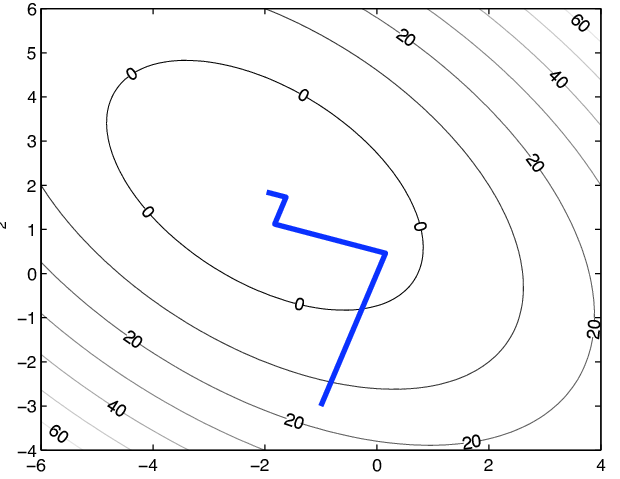
\includegraphics[width=0.5\textwidth]{steepest_descent.png}
	\caption{Metoda Gradientului Descendent}
	\label{fig:1}
\end{figure}

\begin{algorithm}
	\caption{Metoda Gradientului Descendent}
	\begin{algorithmic}[1]
		\State $r \gets b$
		\State $x \gets 0$
		\State $i \gets 1$
		\While{$i \leq \text{max\_iter}$}
		\If{$\|r\| < \text{tol}$}
		\State \textbf{break}
		\EndIf
		\State $ar \gets A r$
		\State $\alpha \gets \frac{r^T r}{r^T ar}$
		\State $x \gets x + \alpha \cdot r$
		\State $r \gets r - \alpha \cdot ar$
		\State $i \gets i + 1$
		\EndWhile
	\end{algorithmic}
\end{algorithm}

\subsubsection{Metoda Gradientului Conjugat}

O metodă mult mai eficientă este cea a gradientului conjugat, ea având
proprietatea de a converge garantat după cel mult $n$ iterații. Ideea din
spatele acestei metode este de a construi un set de direcții de căutare
conjugate între ele în raport cu matricea $A$. Spre deosebire de metoda
gradientului descendent, unde fiecare direcție de căutare este ortogonală cu cea
anterioară, în metoda gradientului conjugat direcțiile sunt $A-conjugate$, adică
satisfac relația:
\begin{equation*}
	p^{(i)T} A p^{(j)} = 0, \quad \text{pentru } i \neq j.
\end{equation*}

Această proprietate asigură că soluția exactă este atinsă în cel mult $n$ pași
pentru un sistem de dimensiune $n$, în cazul în care nu există erori numerice.

Algoritmul începe similar cu metoda gradientului descendent, însă în loc să ne
deplasăm în direcția dată de gradient, construim un nou vector $p^{(k)}$ care
este conjugat cu toate cele anterioare (Gram-Schmidt):
\begin{equation*}
	p^{(k)} = r^{(k)} + \sum_{i=0}^{k-1} \beta^{(i)} p^{(i)}
\end{equation*}

Știm de la laboratorul 3 că procesul Gram-Schmidt nu este unul eficient. Totuși,
se pare că este suficient să calculăm doar pe $\beta^{(k)}$ pentru a obține
direcții conjugate.

\textbf{Subspații Krylov.} Subspațiul de dimensiune $k$ îl generăm ca fiind
\begin{equation*}
	K_k = \text{span}\{r^{(0)}, Ar^{(0)}, A^2 r^{(0)}, \ldots, A^{k-1} r^{(0)}\}
\end{equation*}

Dacă $A$ este inversabilă atunci folosind teorema Cayley-Hamilton, toți vectorii
din $K_k$ sunt liniari independenți. Se poate observa că $r^{(0)}$ și $p^{(k)}$
progresează în același subspațiu Krylov. Având în vedere că la pasul $k$,
vectorul $r$ avansează în subspațiul Krylov $K_k$, scăzând din el proiecția
acestuia pe vectorii $p$ calculați anterior din subspațiul $K_{k-1}$, rămânem
doar cu componenta corespunzătoare lui $\beta_k$. Gândiți-vă la algoritmul
Gram-Schmidt modificat: la fiecare iterație scădem din toți vectorii proiecțile
lor vectorul curent.

Coeficientul $\beta^{(k)}$ este
\begin{equation*}
	\beta^{(k)} = -\frac{\mathbf{r}^{(k)T} A \mathbf{p}^{(k-1)}}{\mathbf{p}^{(k-1)T} A \mathbf{p}^{(k-1)}}
\end{equation*}

Iar după ce se prelucrează se ajunge la formula lui $\beta$:
\begin{equation*}
	\beta^{(k)} = \frac{r^{(k)T} r^{(k)}}{r^{(k-1)T} r^{(k-1)}}
\end{equation*}

\begin{algorithm}
	\caption{Metoda Gradientului Conjugat}
	\begin{algorithmic}[1]
		\State $r \gets b$
		\State $p\gets r$
		\State $x \gets 0$
		\State $i \gets 1$
		\While{$i \leq \text{max\_iter}$}
		\State $ap \gets A p$
		\State $pap \gets p^T ap$
		\State $rr \gets r^T r$

		\State $\alpha \gets \frac{rr}{pap}$
		\State $x \gets x + \alpha\cdot p$
		\State $r \gets r - \alpha \cdot ap$
		\If{$\|r\| < \text{tol}$}
		\State \textbf{break}
		\EndIf
		\State $\beta \gets \frac{r^T r}{rr}$
		\State $p \gets r + \beta \cdot p$
		\State $i \gets i + 1$
		\EndWhile
	\end{algorithmic}
\end{algorithm}

\begin{figure}[ht]
	\centering
	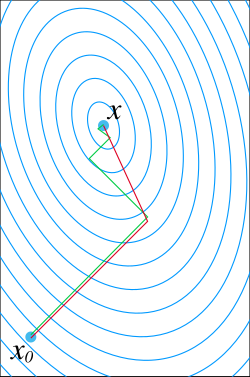
\includegraphics[width=0.3\textwidth]{conjugate_vs_steepest.png}
	\caption{Metoda Gradientului Conjugat și a Gradientului Descendent}
	\label{fig:2}
\end{figure}

\subsection{Sisteme de ecuații neliniare}
Un sistem de ecuaţii neliniare are forma:
\begin{align*}
	 & f_{1}(x_{1},x_{2},x_{3},...,x_{n-1},x_{n})=0 \\
	 & f_{2}(x_{1},x_{2},x_{3},...,x_{n-1},x_{n})=0 \\
	 & ...                                          \\
	 & f_{n}(x_{1},x_{2},x_{3},...,x_{n-1},x_{n})=0 \\
\end{align*}

$f_{i}$ reprezintă funcţii cunoscute de $n$ variabile $x_{1}, x_{2}, ..., x_{n}$,
presupuse continue, împreună cu derivatele lor parţiale până la un ordin
convenabil (de obicei, până la ordinul doi). Se va urmări găsirea soluţiilor
reale ale sistemului într-un anumit domeniu de interes, domeniu în care se
consideră valabile proprietăţile de continuitate impuse funcţiilor
$f_{i}$ şi derivatelor lor. Rezolvarea sistemului este un proces iterativ în
care se porneşte de la o aproximaţie iniţială pe care algoritmul o va îmbunătăţi
până ce se va îndeplini o condiţie de convergenţă. În cazul de faţă, localizarea
apriori a soluţiei nu mai este posibilă (nu există o metodă analoagă metodei
înjumătăţirii intervalelor).

\subsubsection{Puncte fixe}

Și în acest caz putem încerca să transformăm sistemul de ecuații neliniare
într-un sistem de ecuații de tip punct fix:
\begin{align*}
	 & x_{1} = g_{1}(x_{1},x_{2},x_{3},...,x_{n-1},x_{n}) \\
	 & x_{2} = g_{2}(x_{1},x_{2},x_{3},...,x_{n-1},x_{n}) \\
	 & ...                                                \\
	 & x_{n} = g_{n}(x_{1},x_{2},x_{3},...,x_{n-1},x_{n}) \\
\end{align*}

Pentru ca funcțiile $g_{i}$ să fie contracții avem nevoie ca gradienții lor să
aibă normă mai mică decât 1 pe domeniul ales.

\subsubsection{Metoda Newton}

Pentru simplificarea notaţiei, considerăm
$F=\left(\begin{array}{c}f_{1}\\f_{2}\\f_{3}\\...\\f_{n} \end{array}\right)$ şi
$x=(x_{1},x_{2},...,x_{n})$. Sistemul îl putem rescrie ca $F(x)=0$.
Notăm cu $x^{(k)}$ estimarea la pasul $k$ a soluţiei $x^{*}$, deci $F(x^{*})=0$.

Se poate deduce relaţia:
$$x^{(k+1)} = x^{(k)} - J(x^{(k)})^{-1}F(x^{(k)}), k=0,1,2,... $$

\noindent  unde $J$ este matricea \textit{Jacobiană}
\[J=  \left( \begin{array}{ccc}
			\frac{\partial F_{1}}{ \partial x_{1}} & ...   & \frac{\partial F_{1}}{ \partial x_{n}} \\
			{...}                                  & {...} & {...}                                  \\
			\frac{\partial F_{n}}{ \partial x_{1}} & ...   & \frac{\partial F_{n}}{ \partial x_{n}}
		\end{array} \right)\]

Dacă matricea $J$ este neinversabilă, atunci pasul este nedefinit. Vom presupune
că $J(x^*)$ este inversabilă, iar continuitatea lui $J$ va asigura că
$J(x^{(k)})$ este inversabilă pentru orice $x^{(k)}$ suficient de apropiat de
$x^*$. Secvenţa definită iterativ converge spre soluția $x^*$.
Condiţia de oprire la iteraţia $k$, $\left \|x^{*}-x^{(k)}  \right \|<tol$, unde
$tol$ este o toleranţă dată, se poate arăta că revine la
$\left \|x^{(k)}-x^{(k-1)}  \right \|<tol.$

\subsection{Polinoame}

\subsubsection{Rădăcinile polinoamelor}

Fie $p$ un polinom de grad $n$,
$p(x)= a_{n}x^{n}+a_{n-1}x^{n-1}+a_{n-2}x^{n-2}+...+a_{1}x+a_{0}$, cu
$a_{n}\neq 0$. Conform cu \textit{teorema fundamentală a algebrei}, polinomul
$p$ are $n$ rădăcini reale sau complexe (numărând şi multiplicităţile). În cazul
în care coeficienţii $a_{i}$ sunt toţi reali,  rădăcinile complexe apar
conjugate (de forma $c+id$ şi $c-id$).

Folosind regula semnelor a lui Descartes, putem număra câte rădăcini reale
pozitive are polinomul $p$. Fie $v$ numărul variaţiilor de semn ale
coeficienţilor $a_{n}, a_{n-1}, a_{n-2},.., a_{1},a_{0}$, ignorând coeficienţii
care sunt nuli. Fie $n_{p}$ numărul de rădăcini pozitive. Avem următoarele două
relaţii:
\begin{enumerate}
	\item $n_{p}\leq v$;
	\item $v-n_{p}$ este un număr par.
\end{enumerate}

Analog, numărul de rădăcini reale negative ale lui $p(x)$ se obţine folosind numărul de schimbări de semn ale coeficienţilor polinomului  $p(-x)$.
Pentru determinarea rădăcinilor, se pot aplica metodele descrise anterior la punctul $b)$, dacă nu se cunoaşte localizarea rădăcinilor pe intervale.

\subsubsection{Lucrul cu polinoame în MATLAB}

În MATLAB, un polinom este reprezentat prin coeficienţii săi (în ordine descrescătoare). Vectorul \verb|p = [-2, -1, 0, 1, 2]| reprezintă polinomul $-2x^{4}-x^{3}+x+2$.

\textbf{Funcții MATLAB}
\begin{itemize}
	\item \verb|polyval(p, x)| - calculează $p(x)$.
	\item \verb|conv(p, q)| - calculează convoluția celor două polinoame (le înmulțește).
	\item \verb|polyder(p)| - calculează derivata polinomului.
	\item \verb|polyint(p)| - calculează integrala polinomului.
\end{itemize}

\section{Probleme propuse}

\begin{questions}

	\question Să se determine tipul (dacă sunt reale pozitive sau negative,
	complexe) rădăcinilor polinomului $p(x)=3x^{6}+x^{4}-2x^{3}-5$.

	\question Să se rezolve următorul sistem prin puncte fixe:
	\begin{align*}
		 & \frac{x}{2} + \frac{1}{4}\ln(1 + y)   = 2 \\
		 & \frac{y}{4} + \frac{1}{10}\arctan(x)  = 2
	\end{align*}

	\question Să se scrie în MATLAB un program care rezolvă un sistem de ecuaţii
	neliniare prin metoda Newton. Ca intrare, se consideră un vector coloană care
	reprezintă $x^{(0)}$, un pointer (handler) la o funcţie care evaluează $F$
	într-un vector generic $x$, un pointer la o funcţie care calculează Jacobiana
	într-un vector generic $x$, o toleranţă dată $\epsilon$. Metoda se opreşte
	atunci când  $\left \| x^{(k)}-x^{(k-1)} \right \|< \epsilon$ şi returnează
	vectorul soluţie $x^{*}$ şi numărul de iteraţii $n$ care au fost necesare pentru
	producerea soluţiei.

\end{questions}

\bibliographystyle{plain}
\bibliography{refs}
\end{document}
